\PassOptionsToPackage{unicode}{hyperref}
\PassOptionsToPackage{hyphens}{url}

\documentclass[
]{article}
\usepackage{amsmath,amssymb}
\usepackage{lmodern}
\usepackage{iftex}
\ifPDFTeX
  \usepackage[T1]{fontenc}
  \usepackage[utf8]{inputenc}
  \usepackage{textcomp} 
\else 
  \usepackage{unicode-math}
  \defaultfontfeatures{Scale=MatchLowercase}
  \defaultfontfeatures[\rmfamily]{Ligatures=TeX,Scale=1}
\fi

\IfFileExists{upquote.sty}{\usepackage{upquote}}{}
\IfFileExists{microtype.sty}{
  \usepackage[]{microtype}
  \UseMicrotypeSet[protrusion]{basicmath} 
}{}
\makeatletter
\@ifundefined{KOMAClassName}{
  \IfFileExists{parskip.sty}{
    \usepackage{parskip}
  }{
    \setlength{\parindent}{0pt}
    \setlength{\parskip}{6pt plus 2pt minus 1pt}}
}{
  \KOMAoptions{parskip=half}}
\makeatother
\usepackage{xcolor}
\usepackage{graphicx}
\makeatletter
\def\maxwidth{\ifdim\Gin@nat@width>\linewidth\linewidth\else\Gin@nat@width\fi}
\def\maxheight{\ifdim\Gin@nat@height>\textheight\textheight\else\Gin@nat@height\fi}
\makeatother

\setkeys{Gin}{width=\maxwidth,height=\maxheight,keepaspectratio}

\makeatletter
\def\fps@figure{htbp}
\makeatother
\setlength{\emergencystretch}{3em}  
\providecommand{\tightlist}{
  \setlength{\itemsep}{0pt}\setlength{\parskip}{0pt}}
\setcounter{secnumdepth}{-\maxdimen} 
\ifLuaTeX
  \usepackage{selnolig}  
\fi
\IfFileExists{bookmark.sty}{\usepackage{bookmark}}{\usepackage{hyperref}}
\IfFileExists{xurl.sty}{\usepackage{xurl}}{} 
\urlstyle{same}
\hypersetup{
  hidelinks,
  pdfcreator={LaTeX via pandoc}}
\author{}
\date{}

\begin{document}
\begin{quote}
\centering
\title{tire-pressure-sensor}
\hypertarget{tire-pressure-sensor}{%
\section{Tire Pressure Sensor}\label{tire-pressure-sensor}}
\end{quote}

\begin{quote}
\centering
\textbf{\hypertarget{mini-project-final-report}{MINI PROJECT FINAL REPORT}}
\end{quote}

\begin{quote}
\centering
\textbf{Automobile Electronics}
\end{quote}

\begin{quote}
\centering
\textbf{TEE3310}
\end{quote}



\vfill
\hypertarget{group-members}{%
\paragraph{Group Members:}\label{group-members}}

\begin{enumerate}
\def\labelenumi{\arabic{enumi}.}
\item
  \begin{quote}
  D.M.A.L. Dissanayake - 21UG0570
  \end{quote}
\item
  \begin{quote}
  T.V. Wijesinghe - 21UG0080
  \end{quote}
\end{enumerate}
\vfill
\begin{quote}
\centering
Faculty of Technology

Sri Lanka Technological Campus
\vfill
January 2024
\newpage

\end{quote}

\hypertarget{content}{%
\section{CONTENT}\label{content}}

\protect\hyperlink{key-words}{KEY WORDS}.................................................................................... 03

\protect\hyperlink{acknowledgement}{ACKNOWLEDGEMENT}................................................................... 03

\protect\hyperlink{key-words}{ABSTRACT}........................................................................................ 04

\protect\hyperlink{abstract}{CHAPTER 01}

\protect\hyperlink{background-to-the-project}{BACKGROUND TO THE PROJECT}
................................................05

\protect\hyperlink{project-description}{PROJECT DESCRIPTION} .................................................................05

\protect\hyperlink{project-aim}{PROJECT AIM} ....................................................................................05

\protect\hyperlink{_bookmark7}{OBJECTIVES} .......................................................................................05

\protect\hyperlink{_bookmark8}{CHAPTER 02}

\protect\hyperlink{traditional-direct-tpms}{TRADITIONAL DIRECT TPMS} .........................................................06

\protect\hyperlink{indirect-tpms}{INDIRECT TPMS} ................................................................................06

\protect\hyperlink{chapter-02}{ADVANCE TPM} ...................................................................................07

\protect\hyperlink{communication-technologies}{COMMUNICATION
TECHNOLOGIES} ...............................................07

\protect\hyperlink{advance-tpm}{EMERGING TECHNOLOGIES} ............................................................08

\protect\hyperlink{emerging-technologies}{CHAPTER 03} ........................................................................................09

\protect\hyperlink{_bookmark15}{CHAPTER 04}

\protect\hyperlink{implementation}{IMPLEMENTATION} .............................................................................10

\protect\hyperlink{results-and-analysis}{RESULTS AND ANALYSIS} ...................................................................11

\protect\hyperlink{chapter-05}{CHAPTER 05}

\protect\hyperlink{conclusion}{CONCLUSION} ........................................................................................12

\protect\hyperlink{future-work}{FUTURE WORK} ....................................................................................12

\protect\hyperlink{appendices}{APPENDICES} .........................................................................................13

\protect\hyperlink{chapter-05}{REFERENCES}..........................................................................................18

\newpage

\hypertarget{key-words}{%
\subsubsection{KEY WORDS}\label{key-words}}

\begin{quote}
Esp 32 micro controller, BMP 180 pressure sensor, dot board, Arduino,
programming, LED Display.
\end{quote}

\hypertarget{acknowledgement}{%
\paragraph{ACKNOWLEDGEMENT}\label{acknowledgement}}

\begin{quote}
We express our sincere gratitude to all those who contributed to the
successful completion of this tire pressure monitoring project. First
and foremost, we extend our heartfelt appreciation to our project
supervisor for their guidance, invaluable insights, and unwavering
support throughout the entire duration of this endeavor. We would like
to thank the faculty members who provided assistance and resources,
fostering an environment conducive to learning and innovation. Special
thanks go to our peers and colleagues for their collaboration and shared
enthusiasm, creating a dynamic and inspiring atmosphere.

Furthermore, we are grateful for the technical expertise and support
received from professionals in the field, as well as for the facilities
and equipment provided that were integral to the
project\textquotesingle s execution. Last but not least, we extend our
deepest appreciation to our family and friends for their encouragement
and understanding during the project, as their unwavering support played
a significant role in the successful realization of this endeavor.
\end{quote}

\newpage
\hypertarget{abstract}{%
\subsubsection{ABSTRACT}\label{abstract}}

\begin{quote}
This project introduces an innovative Tire Pressure Monitoring System
(TPMS) designed to enhance vehicle safety and maintenance. The system
incorporates a BMP180 pressure sensor to measure both tire pressure and
temperature, with data relayed to an ESP32 microcontroller. Utilizing
Wi-Fi connectivity, the ESP32 transmits these values to an LED display
in real-time, offering users a convenient means of monitoring tire
conditions. A crucial safety feature includes an alert mechanism
triggered when pressure values fall below a predefined threshold,
signaling a potential tire leak. The project aims to contribute to road
safety by providing immediate feedback to users and facilitating timely
maintenance interventions. Future work may involve the integration of
additional sensors, exploration of advanced communication protocols, and
the incorporation of machine learning algorithms for predictive
maintenance enhancements. This tire pressure monitoring system stands as
a promising solution in the pursuit of safer and more reliable
automotive technologies.

\newpage
\hypertarget{chapter-01}{%
\subsection{CHAPTER 01}\label{chapter-01}}
\end{quote}

\hypertarget{background-to-the-project}{%
\subsubsection{BACKGROUND TO THE
PROJECT}\label{background-to-the-project}}

\begin{quote}
In modern automobiles, maintaining proper tire pressure is critical for
safety, fuel efficiency, and overall performance. The use of Tire
Pressure Sensors has become a regular element in vehicle technology.
This project intends to create and improve a Tire Pressure Sensor system
that not only monitors tire pressure but also sends real-time data to
the vehicle\textquotesingle s central control unit.
\end{quote}

\hypertarget{project-description}{%
\subsubsection{PROJECT DESCRIPTION}\label{project-description}}

\begin{quote}
This project involves the design, development, and implementation of an
advanced sensor system. The system will be capable of accurately
measuring tire pressure and communicating this data to the
vehicle\textquotesingle s onboard computer. The project will encompass
both hardware and software components, ensuring seamless integration
with existing vehicle systems.
\end{quote}

\hypertarget{project-aim}{%
\subsubsection{PROJECT AIM}\label{project-aim}}

\begin{quote}
The aim of this project is to design and implement a tire monitoring
system that continuously measures and analyzes tire sensor data to
detect and alert users to the presence of any leaks. The primary goal is
to enhance vehicle safety and performance by providing real-time,
proactive information on tire conditions. The system will employ
advanced sensor technology to monitor tire pressure, temperature, and
other relevant parameters, ensuring early detection of leaks that may go
unnoticed by conventional visual inspections. Through continuous data
analysis and timely notifications, the project aims to prevent potential
tire-related incidents, reduce the risk of unexpected breakdowns, and
contribute to overall road safety\protect\hypertarget {_bookmark7}{}{}y.
\end{quote}

\hypertarget{objectives}{%
\subsubsection{OBJECTIVES}\label{objectives}}

\begin{itemize}
\item
  \begin{quote}
  Achieve a precision level of tire pressure measurement within a ±1\%
  margin of error. Establish a communication range of at least 10 meters
  between sensors and the central control unit.
  \end{quote}
\item
  \begin{quote}
  Calculate if the tire is having an undetectable leak to the naked
  eye\protect\hypertarget{_bookmark8}{}{}.
  \end{quote}
\end{itemize}
\newpage
\hypertarget{chapter-02}{%
\subsection{CHAPTER 02}\label{chapter-02}}

\hypertarget{traditional-direct-tpms}{%
\subsubsection{TRADITIONAL DIRECT TPMS}\label{traditional-direct-tpms}}

\begin{quote}
The Traditional Direct TPMS employs a methodology wherein pressure
sensors situated within each tire wirelessly transmit data to a central
receiver located in the vehicle. This system utilizes piezoelectric
pressure sensors and radio frequency (RF) communication technology,
enabling highly accurate and real-time monitoring of tire pressure,
along with individual tire identification capabilities. Despite its
strengths in providing precise data, the Traditional Direct TPMS has
notable weaknesses, including relatively high costs, the need for
installation, and periodic battery replacements. Furthermore, it is
susceptible to signal interference. Insights from recent literature
highlight ongoing research efforts focused on optimizing sensor size and
power consumption, refining communication protocols, and incorporating
additional diagnostics such as temperature and tread wear into the
system for a more comprehensive monitoring approach.
\end{quote}

\hypertarget{indirect-tpms}{%
\subsubsection{INDIRECT TPMS}\label{indirect-tpms}}

\begin{quote}
Indirect TPMS operates by utilizing the existing Anti-lock Braking
System (ABS) sensors to monitor variations in wheel rotation speed,
indirectly deducing changes in tire pressure. This system relies on the
technology of existing ABS sensors and involves the analysis of wheel
speed data. Notably, its strengths lie in being a cost-effective
solution that requires no installation or ongoing maintenance, and it
remains operational even in the presence of flat tires. However, it
comes with inherent weaknesses, including lower accuracy in comparison
to direct TPMS, an inability to identify individual tire pressure
issues, and susceptibility to external factors such as road conditions.
Current literature insights in this domain focus on developing
algorithms to enhance pressure estimation accuracy, integrating
additional sensors like accelerometers into the system, and exploring
ways to integrate Indirect TPMS with traditional TPMS for a more
comprehensive and reliable tire monitoring approach.
\end{quote}

\newpage
\hypertarget{advance-tpm}{%
\subsubsection{ADVANCE TPM}\label{advance-tpm}}

\begin{quote}
Advanced TPMS integrates direct pressure sensors with additional sensors
to measure parameters such as temperature, tread depth, and occasionally
vibration. This system relies on multi-sensor modules and employs
advanced data analysis algorithms for a comprehensive assessment of tire
health. Offering valuable insights, Advanced TPMS enables predictive
maintenance, contributing to enhanced safety and fuel efficiency.
However, it comes with certain drawbacks, including being the most
expensive option in the TPMS spectrum and requiring complex installation
and data management. Recent literature in this field emphasizes research
on miniaturizing and seamlessly integrating sensors into tire systems,
developing self-healing tire materials, and harnessing AI- powered
predictive models for early detection of potential issues, showcasing
the ongoing efforts to refine and optimize Advanced TPMS technologies.
\end{quote}

\hypertarget{communication-technologies}{%
\subsubsection{COMMUNICATION
TECHNOLOGIES}\label{communication-technologies}}

\begin{quote}
Various communication technologies play crucial roles in tire pressure
monitoring systems (TPMS). Bluetooth, with its short-range and low-power
attributes, facilitates data transmission between sensors and receivers
within the vehicle. On the other hand, Radio Frequency (RF) offers a
longer range, making it reliable for both in-vehicle and short-range
remote monitoring applications. Cellular connectivity emerges as a
powerful option, allowing remote monitoring and alerts even when the
vehicle is parked, which proves invaluable for fleet management
scenarios. Current literature trends in this domain focus on enhancing
the security of communication protocols, integrating TPMS with cloud
platforms for efficient data storage and analysis, and exploring the
potential of low-power, wide-area network (LPWAN) technologies to extend
range and achieve cost-effectiveness in tire monitoring systems. These
insights underscore the ongoing efforts to advance the communication
aspects of TPMS for improved functionality and reliability.
\end{quote}

\newpage
\hypertarget{emerging-technologies}{%
\subsubsection{EMERGING TECHNOLOGIES}\label{emerging-technologies}}

\begin{quote}
Innovative technologies are driving the forefront of TPMS development,
promising substantial advancements in tire safety and management.
Solar-powered sensors represent a notable breakthrough, eliminating the
need for battery replacements and significantly extending the
system\textquotesingle s lifespan. This not only reduces maintenance
efforts but also contributes to sustainable and eco-friendly practices.
Another groundbreaking feature is the integration of self-healing
punctures, where the system autonomously seals small punctures,
enhancing safety and convenience for vehicle operators. Additionally,
the incorporation of AI-powered predictive maintenance is transforming
the landscape by analyzing sensor data to foresee potential issues and
provide timely recommendations for preventative actions. These
cutting-edge developments underscore the potential for a future where
TPMS technologies not only ensure tire safety but also contribute to
overall efficiency and longevity in vehicle maintenance.
\end{quote}
\newpage
\hypertarget{chapter-03}{%
\subsection{CHAPTER 03}\label{chapter-03}}

\begin{quote}
In this methodology, the initial step involves the utilization of the
BMP180 pressure sensor to measure both the pressure and temperature
within the tire. This sensor gathers accurate data reflecting the
internal conditions of the tire {[}1{]}. Subsequently, the gathered
pressure and temperature values are transmitted to the ESP32
microcontroller, which acts as the central processing unit for the
system {[}3{]}.

The ESP32, equipped with Wi-Fi capabilities, facilitates the wireless
transmission of these values to an LED display. This real-time display
allows users to monitor the current pressure and temperature status of
the tire conveniently. The system is designed with a safety feature
wherein if the measured values decrease beyond a predetermined
threshold, indicating a potential leak in the tire, the ESP32 triggers
an indication mechanism.

This alert will be visual through and LED light, to promptly notify the
user of the tire\textquotesingle s compromised condition, enabling
timely intervention and maintenance. In essence, this integrated system
offers a comprehensive solution for monitoring tire pressure and
temperature, ensuring user awareness and enhancing overall vehicle
safety {[}2{]}\protect\hypertarget{_bookmark15}{}{}.
\end{quote}
\newpage
\hypertarget{chapter-04}{%
\subsection{CHAPTER 04}\label{chapter-04}}

\hypertarget{implementation}{%
\subsubsection{IMPLEMENTATION}\label{implementation}}

\begin{quote}
Connect the tire pressure sensors to the ESP32 development board. The
specific wiring will depend on the type of sensor you are using (analog
or digital).Connect any additional components, such as a display unit or
power supply. Ensure that the power supply can provide sufficient power
for both the ESP32 and the tire pressure sensors. Write code to read
data from each tire pressure sensor. This may involve using analog or
digital pins on the ESP32, depending on the sensor type. Convert the
sensor readings to actual pressure values using the
sensor\textquotesingle s specifications. Implement code to transmit the
tire pressure data wirelessly using the ESP32\textquotesingle s Wi-Fi or
Bluetooth capabilities. For Wi-Fi communication, you might consider
setting up a simple web server on the ESP32 to serve the tire pressure
data. If using a display unit, write code to display the tire pressure
data. This could be an LCD display connected to the ESP32. Test the
system by deploying it on a vehicle and monitoring the tire pressure
readings. Calibrate the system if necessary to ensure accurate pressure
readings. Ensure that the system does not interfere with the normal
operation of the vehicle. Implement safety features to handle any
failures or errors gracefully. Document the system, including the
hardware and software components, wiring diagrams, and any calibration
procedures.
\end{quote}

\hypertarget{results-and-analysis}{%
\subsubsection{RESULTS AND ANALYSIS}\label{results-and-analysis}}

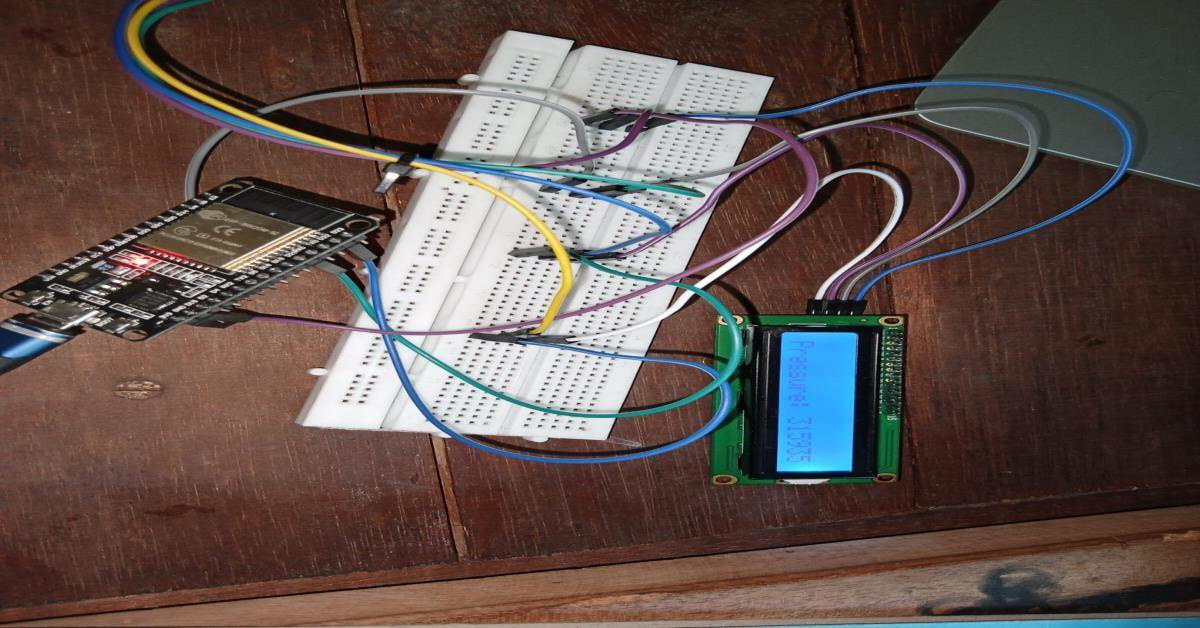
\includegraphics[width=5.31385in,height=3.14in]{image1.jpeg}

\begin{quote}
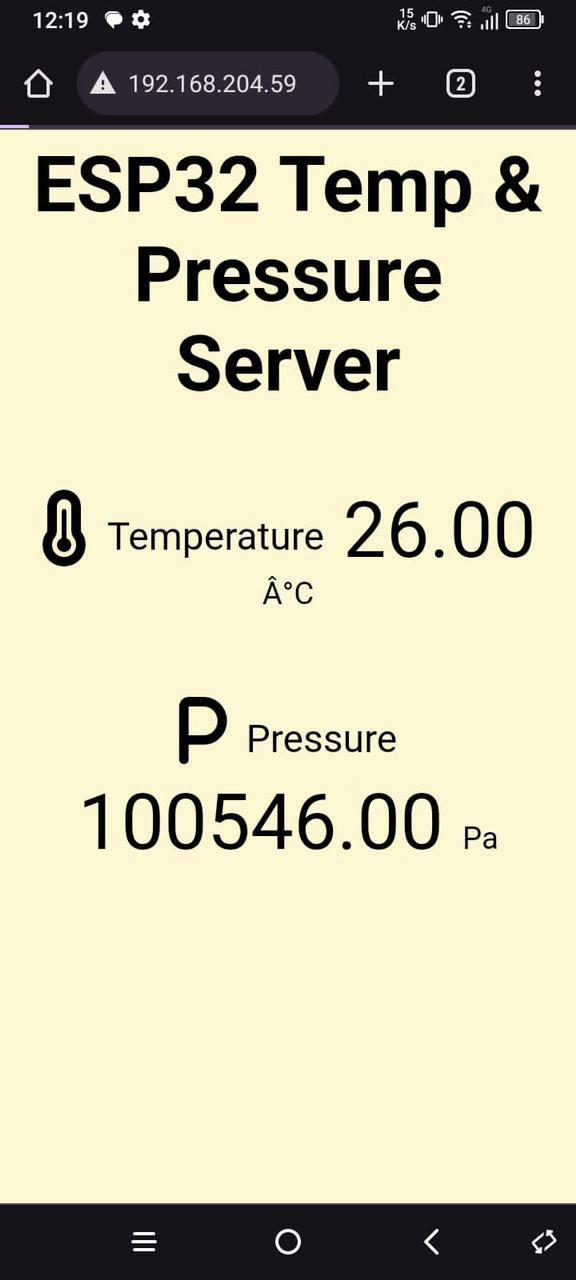
\includegraphics[width=3.59739in,height=4.93333in]{image2.jpeg}
\end{quote}
\newpage
\hypertarget{chapter-05}{%
\subsection{CHAPTER 05}\label{chapter-05}}

\hypertarget{conclusion}{%
\subsubsection{CONCLUSION}\label{conclusion}}

\begin{quote}
In conclusion, the tire pressure monitoring system presented here,
incorporating the BMP180 pressure sensor, ESP32 microcontroller, and LED
display, offers a robust solution for real-time monitoring of tire
conditions. By accurately measuring pressure and temperature within the
tire, the system provides users with immediate feedback through a
wireless connection to the LED display. The implementation of an alert
mechanism ensures timely detection and notification in the event of a
tire leak, contributing to enhanced safety and preventive maintenance.
The integration of such technology into vehicles aligns with the broader
goal of improving road safety and reducing the risks associated with
underinflated or damaged tires.
\end{quote}

\hypertarget{future-work}{%
\subsubsection{FUTURE WORK}\label{future-work}}

\begin{quote}
Moving forward, there are several avenues for future work and
improvement in this tire pressure monitoring project. One potential
focus is the exploration of additional sensor functionalities, such as
incorporating accelerometers or tread wear sensors to provide a more
comprehensive view of tire health. Enhancements in communication
protocols could be pursued to enable integration with mobile
applications for remote monitoring and alerts. Moreover, the integration
of machine learning algorithms could further refine predictive
maintenance capabilities, allowing the system to adapt and improve its
accuracy over time. Additionally, efforts could be directed toward
optimizing power consumption, exploring energy-efficient components, and
possibly investigating alternative power sources beyond the
solar-powered sensors. Continuous research and development in these
areas will contribute to the evolution of tire pressure monitoring
systems, ensuring they remain at the forefront of automotive safety
technology.
\end{quote}
\newpage
\hypertarget{appendices}{%
\subsection{APPENDICES}\label{appendices}}


\begin{minipage}[b]{\linewidth}\raggedright
\begin{quote}
\#include \textless Wire.h\textgreater{}\\
\#include \textless Adafruit\_BMP085.h\textgreater{}\\
\#include \textless WiFi.h\textgreater{}\\
\#include \textless WiFiClient.h\textgreater{}\\
\#include \textless WebServer.h\textgreater{}\\
\#include \textless ESPmDNS.h\textgreater{}\\
\#include \textless LiquidCrystal\_I2C.h\textgreater{}\\
\#include \textless WiFiMulti.h\textgreater{}\\
Adafruit\_BMP085 bmp;\\
\#define ssid1 "XS"\\
\#define password1 "123456789"\\
WiFiMulti wifiMulti;\\
\#define echoPin 2\\
\#define trigPin 4\\
long temperature, pressure;\\
int i = 1;\\
LiquidCrystal\_I2C lcd(0x27, 16, 2);\\
WebServer server(80);
\end{quote}

void handleRoot() \{\\
char msg{[}1500{]};\\

float temp = readTemperature();\\
float press = readPressure();\strut
\end{minipage} \\

\begin{minipage}[b]{\linewidth}\raggedright
\begin{quote}
snprintf(msg, 1500,\\
"\textless html\textgreater\textbackslash{}\\
\textless head\textgreater\textbackslash{}\\
\textless meta http-equiv=\textquotesingle refresh\textquotesingle{}
content=\textquotesingle5\textquotesingle/\textgreater\textbackslash{}\\
\textless meta name=\textquotesingle viewport\textquotesingle{}content=\textquotesingle width=device-width,initial-scale=1\textquotesingle\textgreater\textbackslash{}\\
\textless script
src=\textquotesingle https://kit.fontawesome.com/3e6ef2b5ef.js\textquotesingle{}
crossorigin=\textquotesingle anonymous\textquotesingle\textgreater\textless/script\textgreater\textbackslash{}
\textless title\textgreater ESP32 Distance
Server\textless/title\textgreater\textbackslash{}\\
\textless style\textgreater\textbackslash{}\\
html \{ font-family: Arial; display: inline-block; margin: 0px auto;
text-align: center;\}\textbackslash{} body \{background:
\#FFF7D4;\}\textbackslash{}\\
h2 \{ font-size: 3.0rem; \}\textbackslash{}\\
p \{ font-size: 3.0rem; \}\textbackslash{}\\
.units \{ font-size: 1.2rem; \}\textbackslash{}\\
.dht-labels\{ font-size: 1.5rem; vertical-align:middle; padding-bottom:
15px;\}\textbackslash{}\\
\textless/style\textgreater\textbackslash{}\\
\textless/head\textgreater\textbackslash{}\\
\textless body\textgreater\textbackslash{}\\
\textless h2\textgreater ESP32 Tire pressure
sensor\textless/h2\textgreater\textbackslash{}\\
\textless p\textgreater\textbackslash{}\\
\textless i class=\textquotesingle fa-solid
fa-temperature-three-quarters\textquotesingle\textgreater\textless/i\textgreater\textbackslash{}\\
\textless span
class=\textquotesingle dht-labels\textquotesingle\textgreater Temperature\textless/span\textgreater\textbackslash{}\\
\textless span\textgreater\%.2f\textless/span\textgreater\textbackslash{}\\
\textless span
class=\textquotesingle units\textquotesingle\textgreater{}
°C\textless/span\textgreater\textbackslash{}\\
\textless/p\textgreater\textbackslash{}\\
\textless p\textgreater\textbackslash{}
\end{quote}\strut
\end{minipage} \\

\begin{minipage}[b]{\linewidth}\raggedright
\begin{quote}
\textless i class=\textquotesingle fa-solid
fa-p\textquotesingle\textgreater\textless/i\textgreater\textbackslash{}\\
\textless span
class=\textquotesingle dht-labels\textquotesingle\textgreater Pressure\textless/span\textgreater\textbackslash{}\\
\textless span\textgreater\%.2f\textless/span\textgreater\textbackslash{}\\
\textless span
class=\textquotesingle units\textquotesingle\textgreater{}
Pa\textless/span\textgreater\textbackslash{}\\
\textless/p\textgreater\textbackslash{}\\
\textless/body\textgreater\textbackslash{}\\
\textless/html\textgreater",\\
temp, press\\
);\\
server.send(200, "text/html", msg);\\
\}\\
void setup(void) \{\\
Serial.begin(9600);\\
lcd.init();\\
lcd.backlight();\\
lcd.clear();\\
pinMode(trigPin, OUTPUT);\\
pinMode(echoPin, INPUT);\\
if (!bmp.begin()) \{\\
Serial.println("Could not find a valid BMP180 sensor, check wiring!");
while (1);\\
\}\\
WiFi.mode(WIFI\_STA);\\
wifiMulti.addAP(ssid1, password1);\\
Serial.println("Connecting to WiFi");\\
lcd.setCursor(0, 0);\\
lcd.print("Connecting...");
\end{quote}\strut
\end{minipage} \\



// Wait for connection\\
while (wifiMulti.run() != WL\_CONNECTED) \{\\
Serial.print(".");\\
lcd.setCursor(0, 1);\\
lcd.print("Attempt " + String(i));\\
i += 1;\\
delay(500);\\
\}

// Reset attempt counter\\
i = 1;\\
lcd.clear();\\
Serial.println("Connected to WiFi");\\
Serial.print("IP address: ");\\
Serial.println(WiFi.localIP());\\
lcd.setCursor(0, 0);\\
lcd.print(WiFi.SSID().c\_str());\\
lcd.setCursor(0, 1);\\
lcd.print(WiFi.localIP());\\
if (MDNS.begin("esp32")) \{\\
Serial.println("MDNS responder started");\\
\}\\
server.on("/", handleRoot);\\
server.begin();\\
Serial.println("HTTP server started");\\
\}


\begin{minipage}[b]{\linewidth}\raggedright
\begin{quote}
void loop(void) \{\\
server.handleClient();\\
// delay(2); // You might not need a delay here\\
\}

float readTemperature() \{\\
temperature = bmp.readTemperature();\\
return temperature;\\
\}

float readPressure() \{\\
pressure = bmp.readPressure();\\
return pressure;\\
\}
\end{quote}\strut
\end{minipage} \\


\newpage
\hypertarget{references}{%
\subsection{REFERENCES}\label{references}}

\begin{enumerate}
\def\labelenumi{\arabic{enumi}.}
\item
  \begin{quote}
  barometric pressure sensor. (n.d.). \emph{Science.gov},
  \end{quote}
\end{enumerate}

\begin{quote}
https:/\href{http://www.science.gov/topicpages/b/barometric\%2Bpressure\%2Bsensor}{/www.scienc}e\href{http://www.science.gov/topicpages/b/barometric\%2Bpressure\%2Bsensor}{.gov/topicpages/b/barometric+pressure+sensor.}
\end{quote}

\begin{enumerate}
\def\labelenumi{\arabic{enumi}.}
\setcounter{enumi}{1}
\item
  \begin{quote}
  Maghzin, N. (2023). \emph{Benefits Of Tyre Pressure Monitoring For
  Business Fleet Vehicles.}
  \end{quote}
\end{enumerate}

\begin{quote}
https://linxio.com/tyre-pressure-monitoring/.

{[}3{]} Source, O. (2023). ESP 32.
https:/\href{http://www.mdpi.com/1424-8220/23/15/6739}{/www.mdpi.com/1424}-\href{http://www.mdpi.com/1424-8220/23/15/6739}{8220/23/15/6739.}
\end{quote}

\end{document}


